\documentclass[10pt]{standalone}
\usepackage[utf8]{inputenc}
\usepackage{helvet}
\renewcommand{\familydefault}{\sfdefault}
\usepackage{tikz}
\usetikzlibrary{shapes.geometric, arrows.meta, positioning, calc, decorations.pathmorphing, decorations.pathreplacing, fit, shadows, shapes.misc}

% Define colors
\definecolor{emeraldpine}{HTML}{1A4D3E}
\definecolor{harvardcrimson}{HTML}{A51C30}
\definecolor{ethdarkblue}{HTML}{1F407A}
\definecolor{ethpetrol}{HTML}{007A87}
\definecolor{ethbronze}{HTML}{B87333}
\definecolor{ethpurple}{HTML}{5B4B8A}
\definecolor{ink}{HTML}{1A202C}
\definecolor{softink}{HTML}{4A5568}
\definecolor{paleink}{HTML}{A0AEC0}
\definecolor{cardbg}{HTML}{F8FAFC}
\definecolor{shadecolor}{HTML}{F4F6F9}

\begin{document}

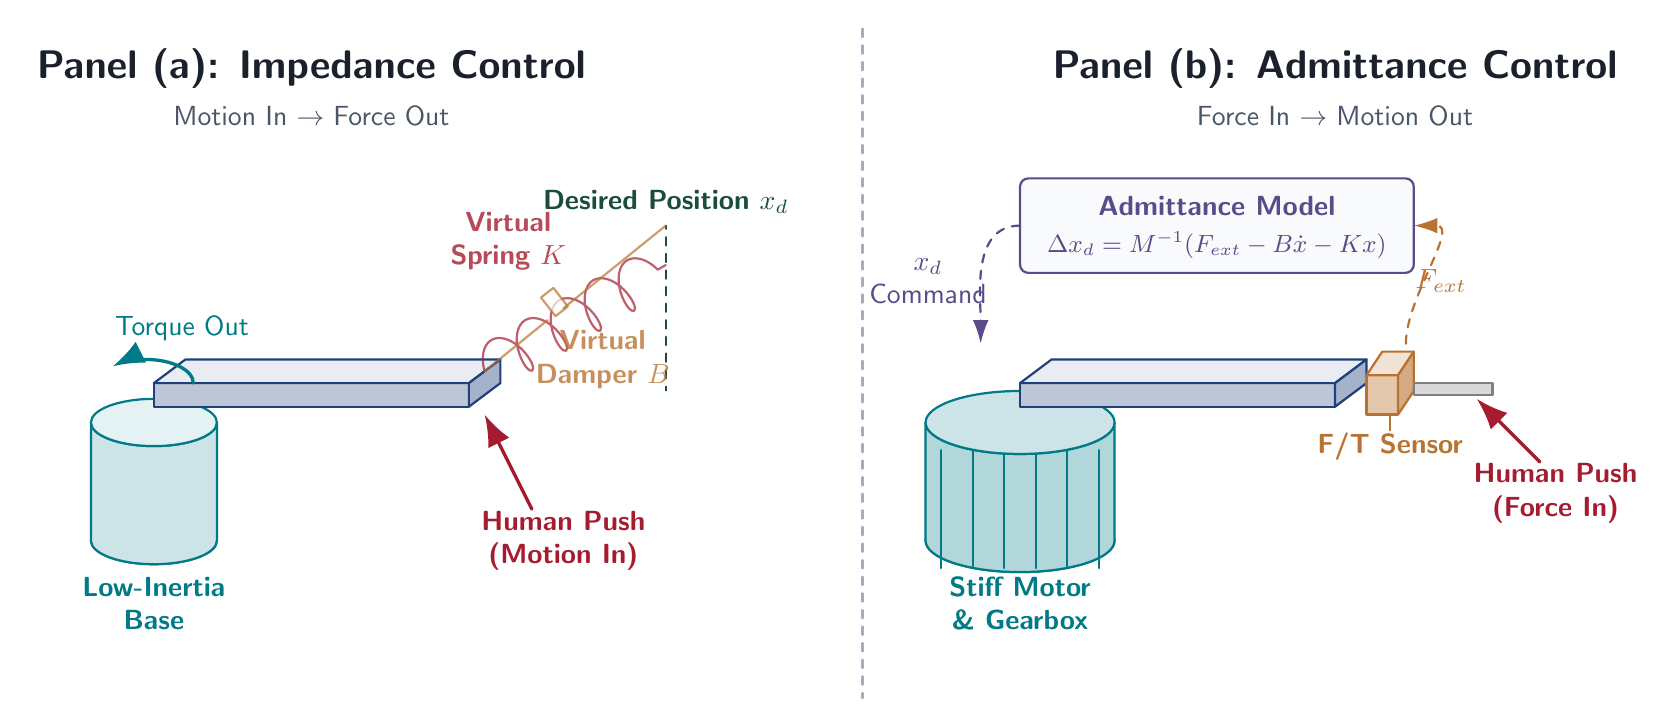
\begin{tikzpicture}[>=Latex, line cap=round, line join=round]

    % Panel (a) Impedance Control
    \begin{scope}[shift={(0,0)}]
        \node[font=\bfseries\Large, text=ink] at (2, 5.5) {Panel (a): Impedance Control};
        \node[font=\normalsize, text=softink] at (2, 4.9) {Motion In $\rightarrow$ Force Out};

        % Motor base (vertical cylinder)
        % bottom ellipse
        \draw[fill=ethpetrol!30, draw=ethpetrol, thick] (0, -0.5) ellipse (0.8 and 0.3);
        % cylinder body
        \draw[fill=ethpetrol!20, draw=ethpetrol, thick] (-0.8, -0.5) -- (-0.8, 1) arc (180:360:0.8 and 0.3) -- (0.8, -0.5) arc (360:180:0.8 and 0.3);
        % top ellipse
        \draw[fill=ethpetrol!10, draw=ethpetrol, thick] (0, 1) ellipse (0.8 and 0.3);
        
        \node[font=\bfseries, text=ethpetrol, align=center] at (0, -1.3) {Low-Inertia\\Base};

        % Robotic Link (pseudo-3D extending right)
        % front face
        \draw[fill=ethdarkblue!30, draw=ethdarkblue, thick] (0, 1.2) rectangle (4, 1.5);
        % top face
        \draw[fill=ethdarkblue!10, draw=ethdarkblue, thick] (0, 1.5) -- (0.4, 1.8) -- (4.4, 1.8) -- (4, 1.5) -- cycle;
        % right face
        \draw[fill=ethdarkblue!40, draw=ethdarkblue, thick] (4, 1.2) -- (4, 1.5) -- (4.4, 1.8) -- (4.4, 1.5) -- cycle;

        % Desired equilibrium point
        \draw[emeraldpine, thick, dashed] (6.5, 1.35) -- (6.5, 3.5);
        \node[font=\bfseries, text=emeraldpine, align=center] at (6.5, 3.8) {Desired Position $x_d$};
        \node[emeraldpine, fill=white, circle, inner sep=1pt] at (6.5, 1.35) {};

        % Virtual environment (translucent)
        % Spring
        \draw[decorate, decoration={coil, aspect=0.5, segment length=5mm, amplitude=3mm}, harvardcrimson, thick, opacity=0.7] (4.2, 1.65) -- (6.5, 3.0);
        \node[font=\bfseries, text=harvardcrimson, opacity=0.8, align=center] at (4.5, 3.3) {Virtual\\Spring $K$};

        % Damper
        \draw[ethbronze, thick, opacity=0.7] (4.2, 1.65) -- (5.0, 2.3);
        \draw[fill=white, draw=ethbronze, thick, opacity=0.7, rotate around={38:(5.1, 2.35)}] (5.1, 2.35) rectangle (5.3, 2.65);
        \draw[ethbronze, thick, opacity=0.7] (5.2, 2.45) -- (6.5, 3.5);
        \node[font=\bfseries, text=ethbronze, opacity=0.8, align=center] at (5.7, 1.8) {Virtual\\Damper $B$};

        % Human Push (Motion In)
        \draw[-{Latex[length=4mm, width=3mm]}, harvardcrimson, very thick] (4.8, -0.1) -- (4.2, 1.1);
        \node[font=\bfseries, text=harvardcrimson, align=center] at (5.2, -0.5) {Human Push\\(Motion In)};

        % Torque Out
        \draw[-{Latex[length=4mm, width=3mm]}, ethpetrol, very thick] (0.5, 1.5) arc (0:135:0.6 and 0.3) node[pos=0.3, above=2mm] {Torque Out};
    \end{scope}

    % Divider
    \draw[dashed, thick, paleink] (9.0, 6) -- (9.0, -2.5);

    % Panel (b) Admittance Control
    \begin{scope}[shift={(11,0)}]
        \node[font=\bfseries\Large, text=ink] at (4, 5.5) {Panel (b): Admittance Control};
        \node[font=\normalsize, text=softink] at (4, 4.9) {Force In $\rightarrow$ Motion Out};

        % Motor base (vertical cylinder, wider/stiffer)
        % bottom ellipse
        \draw[fill=ethpetrol!40, draw=ethpetrol, thick] (0, -0.5) ellipse (1.2 and 0.4);
        % cylinder body
        \draw[fill=ethpetrol!30, draw=ethpetrol, thick] (-1.2, -0.5) -- (-1.2, 1) arc (180:360:1.2 and 0.4) -- (1.2, -0.5) arc (360:180:1.2 and 0.4);
        % Gear teeth (vertical lines)
        \foreach \x in {-1.0, -0.6, -0.2, 0.2, 0.6, 1.0} {
            \draw[ethpetrol, thick] (\x, -0.85) -- (\x, 0.65);
        }
        % top ellipse
        \draw[fill=ethpetrol!20, draw=ethpetrol, thick] (0, 1) ellipse (1.2 and 0.4);
        \node[font=\bfseries, text=ethpetrol, align=center] at (0, -1.3) {Stiff Motor\\\& Gearbox};

        % Robotic Link (pseudo-3D extending right)
        % front face
        \draw[fill=ethdarkblue!30, draw=ethdarkblue, thick] (0, 1.2) rectangle (4, 1.5);
        % top face
        \draw[fill=ethdarkblue!10, draw=ethdarkblue, thick] (0, 1.5) -- (0.4, 1.8) -- (4.4, 1.8) -- (4, 1.5) -- cycle;
        % right face
        \draw[fill=ethdarkblue!40, draw=ethdarkblue, thick] (4, 1.2) -- (4, 1.5) -- (4.4, 1.8) -- (4.4, 1.5) -- cycle;

        % F/T Sensor Disc at the end of the link
        % Better F/T sensor representation: an upright disc/box
        \draw[fill=ethbronze!40, draw=ethbronze, thick] (4.4, 1.1) rectangle (4.8, 1.6);
        \draw[fill=ethbronze!20, draw=ethbronze, thick] (4.4, 1.6) -- (4.6, 1.9) -- (5.0, 1.9) -- (4.8, 1.6) -- cycle;
        \draw[fill=ethbronze!60, draw=ethbronze, thick] (4.8, 1.1) -- (4.8, 1.6) -- (5.0, 1.9) -- (5.0, 1.4) -- cycle;
        
        \node[font=\bfseries, text=ethbronze, align=center] at (4.7, 0.7) {F/T Sensor};
        \draw[ethbronze, thick] (4.7, 0.9) -- (4.7, 1.1);

        % End effector handle
        \draw[fill=gray!30, draw=gray, thick] (5.0, 1.35) -- (6.0, 1.35) -- (6.0, 1.5) -- (5.0, 1.5) -- cycle;

        % Human Push (Force In)
        \draw[-{Latex[length=4mm, width=3mm]}, harvardcrimson, very thick] (6.6, 0.5) -- (5.8, 1.3);
        \node[font=\bfseries, text=harvardcrimson, align=center] at (6.8, 0.1) {Human Push\\(Force In)};

        % Admittance Model Box
        \begin{scope}[shift={(2.5, 3.5)}]
            \draw[fill=cardbg, draw=ethpurple, thick, rounded corners=3pt] (-2.5, -0.6) rectangle (2.5, 0.6);
            \node[text=ethpurple, font=\bfseries] at (0, 0.25) {Admittance Model};
            \node[text=ethpurple, font=\small] at (0, -0.25) {$\Delta x_d = M^{-1}(F_{ext} - B\dot{x} - Kx)$};
        \end{scope}

        % Feedback arrows
        % Sensor to Model (F_ext)
        \draw[-{Latex[length=3mm, width=2mm]}, ethbronze, thick, dashed] (4.9, 2.0) to[out=90, in=0] (5.0, 3.5);
        \node[text=ethbronze, right] at (4.9, 2.8) {$F_{ext}$};

        % Model to Motor (x_d)
        \draw[-{Latex[length=3mm, width=2mm]}, ethpurple, thick, dashed] (0, 3.5) to[out=180, in=90] (-0.5, 2.0);
        \node[text=ethpurple, left, align=center] at (-0.3, 2.8) {$x_d$\\Command};

    \end{scope}

\end{tikzpicture}
\end{document}
